\def\year{2019}\relax
%File: formatting-instruction.tex
\documentclass[letterpaper]{article} %DO NOT CHANGE THIS
\usepackage{aaai19}  %Required
\usepackage{times}  %Required
\usepackage{helvet}  %Required
\usepackage{courier}  %Required
\usepackage{url}  %Required
\usepackage{graphicx}  %Required
\usepackage{algorithm}
\usepackage{algpseudocode}
\usepackage{amsmath}
\usepackage{cite}
\frenchspacing  %Required
\setlength{\pdfpagewidth}{8.5in}  %Required
\setlength{\pdfpageheight}{11in}  %Required
%PDF Info Is Required:
  \pdfinfo{
/Title (Investigation of self-play deep reinforcement learning for Tic-Tac-Toe)
/Author (David Zhao)}
\setcounter{secnumdepth}{0}  
 \begin{document}
% The file aaai.sty is the style file for AAAI Press 
% proceedings, working notes, and technical reports.
%
\title{Investigation of self-play deep reinforcement learning for Tic-Tac-Toe}
\author{David Zhao}
\maketitle
\begin{abstract}
  With the recent announcement by Google that they've developed the world's
  strongest chess AI, AlphaZero, with a self-play deep reinforcement learning
  algorithm, the idea of pairing a neural network with a Monte Carlo Tree Search
  algorithm (MCTS) for complex two player board games has become very popular.
  In this paper I attempt to understand how both neural networks and MCTS work
  and how Googled paired them together by attempting to train my own AlphaZero
  for a simpler game and compare how the algorithm compares with an AI that uses
  MCTS alone. I chose to train my version of AlphaZero, uninterestingly named
  BetaZero, on tic-tac-toe. My work shows that MCTS alone can play tic-tac-toe
  and unfortunately, because of a combination of issues, BetaZero didn't perform
  at all as expected. I reflect on my challenges when trying to train BetaZero.
\end{abstract}

\section{Introduction}
  Designing powerful AI's for complex two player games like chess and Go have
  captured the attention of people for many years. Some of the best chess
  engines in the world like Stockfish continue to improve year on year. Recently 
  Google's AlphaZero managed to create a world class AI from a form of self-play
  reinforcement learning called Tabula-Rasa. AlphaZero is differnet
  from how other strong chess engines because AlphaZero only knew the rules of
  the game and was only allowed to play against itself. AlphaZero works by
  combining Monte Carlo tree search (from now on denoted MCTS) and a neural
  network. The Alphazero paper by David Silver et al. describes at a high level
  how they modified MCTS to utilize the insights of the neural network, how they
  architected and trained their network, and how they evaluated a board
  position.\cite{2017arXiv171201815S}
  
  In this work I try to create an AI for tic-tac-toe similar to AlphaZero. Let
  the tic-tac-toe AlphaZero agent be called BetaZero from now on. The
  reason why such a simple game was chosen was because there are readily
  available AIs which play perfectly to test the BetaZero against.
  In fact, because of how simple tic-tac-toe is, a simple MCTS without deep
  learning plays the game perfectly when the MCTS agent is given enough time or
  simulation iterations to think. Another reason why tic-tac-toe was the game of
  choice was because of the hardware limitations faced. AlphaZero was trained on
  Google's infrastructure whereas I am limited to working with my laptop.
  
  I investigate how augmenting a MCTS
  algorithm for tic-tac-toe with deep learning improves MCTS when it is limited
  to only a small number of simulation iterations. I also investigate how many
  fewer simulation iterations BetaZero needs to play perfectly when compared
  with a vanilla MCTS agent.

\section{Monte Carlo Tree Search}
  Monte Carlo Tree Search (MCTS) is a search algorithm used for finding optimal
  decisions in game trees. MCTS determines the best move in a given game state
  by progressively, and asymetrically, exploring the game tree. Upon each
  iteration the algorithm chooses a new node to explore and then randomly plays
  out the game from the new state to get a game outcome.\cite{Browne12asurvey}
  The total score and visits are stored at each explored  state in the tree and
  the best action is the one leads into the state that has the best average
  score. The high level pseudocode for MCTS is
  \begin{algorithm}
  \caption{Generic MCTS}
  \begin{algorithmic}[1]
  \Function{MctsSearch}{$s_0$}

    \State create root node $n_0$ with state $s_0$
    \While {within computation budget}
      \State $v_l \gets $\Call{Tree Policy}{$v_0$}
      \State $\triangle \gets$ \Call{Default Policy}{$s(v_l)$}
      \State \Call{Backup}{$v_l$, $\triangle$}
    \EndWhile
    \State \Return \Call{$a$(BestChild($v_0$))}{}
  \EndFunction
  \end{algorithmic}
  \end{algorithm}

  \noindent
  where 
  \begin{itemize}
    \item $s_0$ is the initial state
    \item $v_l$ is a game state that is reachable from $s_0$
    \item $\triangle$ is the score of the played out game from state $v_l$
    \item $a$(BestChild($v_0)$) is the action from $s_0$ to the next state that
      has the best expected outcome.
  \end{itemize}

  There are  many variations of MCTS and in this case I chose the version of
  MCTS that generates one unvisited node each iteration. At each new unvisited
  node the default policy was to return the score of the game by playing out the
  game randomly. The result of the game, $z$, took on values $\{1, 0, -1\}$ where
  $1$ meant that the player playing in state $v_l$ won, $0$ encoded a draw and
  $-1$ encoded a loss for the player acting in state $v_l$. The Backup function
  updates the nodes in the game tree that were visited in the current iteration.
  At each node the outcome of the game was added to the node's score and the
  node's number of visits is incremented by one.

  In order for MCTS to be effective the tree policy must balance exploration and
  exploitation. Intuitively, the policy must minimize the amount of regret when
  it chooses the action for $s_0$. The UCB1 policy is known to produce an
  expected logarithmic growth in regret without any prior knowledge of the game
  outcomes for each action.
  \[UCB1(v_l) = \overline{X} + c\sqrt{\frac{2\ln{n}}{n_j}}\]
  $\overline{X} = \frac{\texttt{score at $v_l$}}{\texttt{visits to $v_l$}}$
  indicates the expected score of the node $v_l$ in the game tree. $n_j$
  represents the number of visits child $j$ has received and $n$ represents the
  number of visits $v_l$ as received. $c$ is a constant. If a node hasn't been
  visited its $UCB1$ score is set to infinity. The $UCB1$ score balances
  exploitation and exploration because a node with a low visit count will have a
  higher $UCB1$ score compared to another node with a higher visit cound
  (assuming their $\overline{X}$ scores are the same). Therefore the tree policy
  used for MCTS was to choose the child node with the highest $UCB1$ score.

  \section{AlphaZero Neural Network}
  The neural network that AlphaZero used, denoted as $f_\theta(s)$, took in as
  input a game representation and outputted a tuple $(\vec{p}, v)$ where
  $\theta$ are the parameters of the network, $s$ is the game state, $\vec{p}$
  is the policy that the network thinks is optimal at state $s$, and $v \in [-1,
  1]$ is the expected outcome of the game.

  Since AlphaZero was built to play complex board games like Chess, Go, and
  Shogi, they represented these games as a large $N \times N \times (MT + L)$
  stack of images where the image stack is composed of $T$ time steps of
  $M$ planes of size $N\times N$ where each plane represents a board position
  along with $M$ binary feature planes that denoting piece presence.
  \cite{Silver1140} 
  This game
  representation seemed too complicated for a simple game of tic-tac-toe and as
  a result I represented a game position as a flattened $3\times 3$ array. A
  value of $1$ represented the player's piece, a value of $-1$ represented the
  opponent's piece and $0$ represented an empty square on the board.

  Similarly, a much simpler network architecture was chosen compared to the one
  used for AlphaZero however, the chosen architecture had the same high level
  structure as AlphaZero's network. AlphaZero's architecture consisted of three
  parts. For the first part, the body, AlphaZero had 20 rectified,
  batch-normalized covolutional layers. Afterwords the body split to the policy
  and value head. The policy head was composed of an additional convolutional
  layer where the number of filters represented the probabilities of $\vec{p}$.
  The value head added an addition convolution layer to the body, a
  rectified linear layer, and a $tanh$ layer of size 1. For BetaZero (the
  tic-tac-toe agent), I chose a much simpler network architecture because of
  hardware limitations and because tic-tac-toe is much simpler than chess.

  The input to the network is $(X, 9)$ where X is the number of training
  examples. Next the body is composed of two hidden rectified, batch-normalized
  linear layers. This means that the activation function used is
  \[relu(x) = \begin{cases}x & x \ge 0 \\ 0 & x<0\end{cases}\]
  Each hidden layer in the body had 81 hidden units. The policy head added an
  
  the output of the policy head to be a distribution the softmax function was
  applied to the last hidden layer.
  \[softmax(\vec{p_j}) = \frac{e^{p_j}}{ \sum_{k \in p}e^{p_k}}\]
  The value head also adds an addition rectified batch-normalized hidden layer
  with 18 units to the body. Then a 1 unit layer is and the value is the $tanh$
  of the output. Visually, the network for BetaZero looks like
  \begin{figure}[!htb]
    \centering
    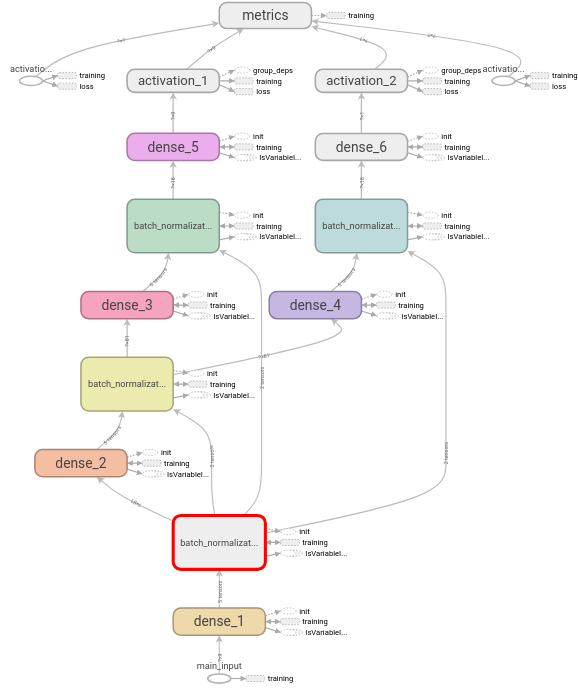
\includegraphics[scale=0.5]{./nn.png} 
    \caption{Network Architecture for BetaZero}
  \end{figure}

  \section{AlphaZero MCTS}
  Since AlphaZero evaluates a given game state by using both an MCTS and the
  neural network described in the previous section. The following changes to
  MCTS are made that differ from what was described in the MCTS section. Even
  though I haven't described how the network is trained, assume for now that
  the network accurately predicts the correct policy vector and game outcome.
  The AlphaZero version of MCTS is
  \begin{algorithm}
  \caption{How AlphaZero finds the best move in a position}
  \begin{algorithmic}[1]
  \Function{AlphaZeroSearch}{$s_0$}

    \State create root node $n_0$ with state $s_0$
    \While {within computation budget}
      \State $v_l \gets $\Call{Tree Policy}{$v_0$}
      \State $\triangle \gets$ \Call{Default Policy}{$s(v_l)$}
      \State \Call{Backup}{$v_l$, $\triangle$}
    \EndWhile
    \State \Return \Call{ComputePolicy$\pi$}{$n_0$}
  \EndFunction
  \end{algorithmic}

  \begin{algorithmic}[1]
  \Function{TreePolicy}{$v_0$}
    \State \Return arg$\max_{v_j}$\Call{ComputeUCB1}{$v_j$}
  \EndFunction
  \end{algorithmic}

  \begin{algorithmic}[1]
  \Function{ComputeUCB1}{$v_0$}
    \State $Q \gets \overline{X}$ 
    \State $c \gets \log{\big(\frac{1+parent.visits+cbase}{cbase}\big)} + cinit$
    \State $U \gets c(prior)\big(\sqrt{\frac{parent.visits}{{1+n}}}\big)$
    \State \Return $Q+U$
  \EndFunction
  \end{algorithmic}

  \begin{algorithmic}[1]
  \Function{DefaultPolicy}{$v_0$}
    \State $\vec{p}, v \gets $\Call{$f$}{$s_0$}
    \State \Return $v$
  \EndFunction
  \end{algorithmic}
  \end{algorithm}

  AlphaZero differs from MCTS in the following ways:
  \begin{itemize}
    \item The default policy for AlphaZero just queries the neural network for
      the value of the game instead of randomly playing out the game.
    \item AlphaZero returns a policy vector $\pi$ instead of the best action.
      For the case in BetaZero, the policy $\pi$ is computed by
      \[p_a = \frac{\overline{X_a} - X_{min}}{\sum_{a\in \text{actions}}
      \overline{X_a}}\quad\quad \forall a\in \text{ valid actions in $s$}\]
    \item AlphaZero augmented the UCB1 score of a node by introducing a $prior$
      parameter. The $prior$ parameter for game state $v_j$ is the probability
      of choosing the action that goes from the parent of state $v_j$ to state
      $v_j$ where the probability is given from the neural network, $f_\theta$. 
  \end{itemize}
  Another smaller addition that Alphazero implemented is that they add some
  noise into the $prior$ probability for each state. More specifically, they
  sample from a gamma distribution and update each probability as follows
  \[prior = \frac{3}{4}prior + \frac{1}{4}noise\]
  The intuition for adding the noise was to make sure that MCTS was properly
  exploring enough in the case that the neural network was tunneled into one
  certain move.

  \section{AlphaZero Training}
  The last component of AlphaZero that needs to be described is how it trains.
  Since Alphazero is only allowed to play against itself, training follows the
  following regime (See algorithm $3$):
  \begin{algorithm}
  \caption{AlphaZero learning process}
  \begin{algorithmic}[1]
    \Function{Train()}{}
    \State create a game with initial state $s \gets s_0$
    \While {the game isn't over}
      \State $\pi \gets $\Call{AlphaZeroSearch}{$s$}
      \State boards, policies $\gets$ \Call{GetTrainingData}{}
      \State $s \gets$ \Call{ChooseMostLikelyMove}{$\pi$}
    \EndWhile
    \State \Call{TrainNeuralNetwork}{boards, policies}
  \EndFunction
  \end{algorithmic}
  \end{algorithm}
  During self-play each position is saved along with the policy $\pi$. At the
  end of the game the outcome of the game, along with the policies $\pi$
  generated during the game are used to train the neural network. The loss
  function for the network is, for a given board state,
  \[\ell = (z-v)^2 - \pi^T\log \vec{p} + c||\theta||^2\]
  $z$ is the outcome of the game of self play. $v$ is the predicted outcome of
  the game for the given board state. $\pi$ is the policy vector returned by the
  AlphaZero MCTS and $\vec{p}$ is the neural network's policy for the given
  board state the last term in the loss function just adds some $\ell_2$
  regularization. This means that the network will try to minimize the mean
  squared loss between the predicted and actual game outcome and it will try to
  minimize the log loss between the predicted and generated policies.
  
  Intuitively, this loss function makes it such that the neural
  network will better predict the outcome of the game from a given board
  position and better predict the best policy from a board position. What is
  interesting is how AlphaZero's MCTS algorithm relies heavily on the neural
  network, $f_\theta$ and so even though neither the network nor MCTS can play
  chess very well the hope is that during each game of self play, the AlphaZero
  augmented MCTS will find a policy that is better than the network's predicted
  policy and that the network's current policy is better than randomly sampling
  the next set of actions. This would allow AlphaZero to slowly and iteratively
  learn how to play the game even though it knew nothing except the rules to
  begin with.

  \section{Differences between Beta and AlphaZero}
  Given that Chess and tic-tac-toe are very different I now list the differences
  I chose to make when building BetaZero. Some of the big design differences are
  already mentioned in the previous section.
  \begin{itemize}
    \item The network BetaZero uses is a much simpler multi output Feed forward
      network compared to AlphaZero's multi output CNN. (See the AlphaZero
      Neural Network section for more info)
    \item I removed the $\ell_2$ regularization from the loss function because
      I thought it added unnecessary complexity.
    \item In the game tree, the score at each node is always with respect to the
      player that is going to move at the root of the tree. This means that when
      a label is generated, by either random play or from BetaZero's value
      prediction, every node's score will be w.r.t to the root player. Therefore
      when running $UCB1$ in nodes with the opposing player, we instead return
      $-Q + U$ instead of $Q+U$. (See psuedocode for reference). This differs
      from AlphaZero where for nodes with the opposing player playing they
      instead add (1-$v$) to that node's score instead of adding just $v$.
    \item Since the tic-tac-toe board has 8 axis' of symmetry, for each board
      position I also added the symmetric boards to the training set with the
      corresponding symmetric policy vectors. Alphazero also used this trick
      when learning how to play Go but didn't do so for chess because there are
      much fewer symmetries on the chess board since queen side castling is
      different from king side castling.
    \item I used a learning rate of $0.02$ whereas in AlphaZero they first
      trained with a learning rate of $0.2$ and decreased it by an order of
      magnitude every $100000$ games.
  \end{itemize}

  \section{Experiments}
  The first thing that I did was to determine how many iterations a regular MCTS
  AI needed to play perfect tic-tac-toe. Since tic-tac-toe is such an easy game,
  I tested whether the MCTS AI played perfectly by personally playing against it
  and then playing the MCTS against itself and making sure that it drew all its
  games. This was achieved for an MCTS that was allowed to search for 750
  iterations. This is an intuitive answer because it means that the AI is
  allowed to approximately look $3$ moves deep which is plenty for enough for
  tic-tac-toe.

  From here I proceed to train BetaZero but limit its MCTS to fewer iterations
  and determine how many fewer (if any) iterations BetaZero needs to play
  perfectly. I trained a BetaZero agent for $20000$ games but noticed that the
  training loss wasn't decreasing much after the first $200$. The loss graph
  looked like
  \begin{figure}[!htb]
    \centering
    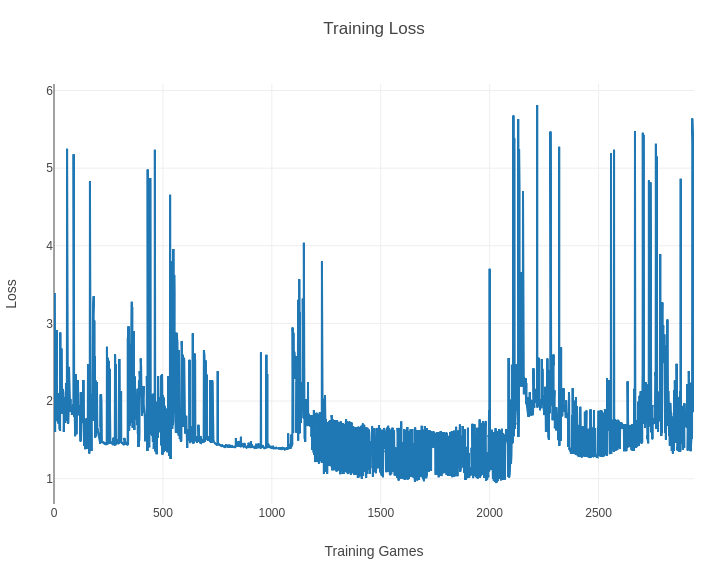
\includegraphics[scale=0.3]{training_loss.png}
    \caption{The training loss of BetaZero during self play}
  \end{figure}
  The concerning thing was that the loss never bottomed out and that while the
  neural network had high accuracy when predicting the expected outcome of the
  game from a given position, it had very low accuracy when predicting the
  policy for a given position. Regardless of the concerning loss graph. I tested
  BetaZero against the perfect MCTS. I tested BetaZero $7$ times. For each test
  I increased BetaZero's MCTS iteration depth. The Beta Zero's iteration depth
  started at $150$ and increased to $750$. Ideally BetaZero would perform
  optimally before it requires a $750$ MCTS iteration depth. I track the draw
  percentage of BetaZero against the optimal MCTS AI. This is calculated simply
  as
  \[\frac{\text{Number of draws}}{\text{Number of total games}}\]
  At each iteration I play $100$ games against the optimal MCTS AI.
  \[\begin{array}{|c|c|}\hline \\ \text{Iterations} & \text{Draw percentage}
    \\\hline
    150 & 0.0 \\
    250 & 0.0 \\
    350 & 0.0 \\
    450 & 0.0 \\
    550 & 0.0 \\
    650 & 0.0 \\
    750 & 0.0 \\
  \hline\end{array}\]
  Because the draw rate was $0.0$ for every version of BetaZero, and since the
  MCTS AI plays perfectly, this meant that BetaZero lost all of its games to the
  regular MCTS AI.

  Unfortunately this result means that something is obviously wrong with
  BetaZero. During troubleshooting I manually evaluated BetaZero against some
  positions and compared the predicted policies and predicted game outcomes with
  a regular MCTS AI. Here are the most interesting results
  \[\begin{array}{c|c|c} & & O \\\hline & X & \\\hline X & O &\end{array}\]
  Here BetaZero correctly classifies the position with a expected game score of
  $0.943$ and the predicted policy $\vec{p}$ is
  \[\begin{array}{c|c|c}0.176 & .153 & 0.001 \\\hline 0.278 & 0.0088 & 0.2086
  \\\hline 0.004 & 0.0023 & 0.167\end{array}\]
  This shows that BetaZero has correctly identified that if a square is taken
  then the probability of taking that invalid action is very low. Also the best
  move BetaZero wants to make is indeed a winning move.

  Here is another example of BetaZero classifying a given position
  \[\begin{array}{c|c|c} O & X & O \\\hline X & X & O\\\hline O & O &
  X\end{array}\]
  The position is clearly a draw but BetaZero estimates that the game score is
  $0.999$.

  Another alarming classification is for the following boards
  \[\begin{array}{c|c|c} & &  \\\hline &  & \\\hline  &  &\end{array}\]
  \[\begin{array}{c|c|c} & &  \\\hline & O & \\\hline  &  &\end{array}\]
  BetaZero predicts that the expected outcome of the empty board is $0.92$ which
  is way too high given that the expected the outcome, with perfect play is $0$.
  It predicts the expected outcome for the second board is $-0.98$ which is too
  pessimistic.

  From manually debugging BetaZero, it is clear that it correctly predicts the
  outcome and policy of some positions while for others it is wrong. This leads
  me to believe there is either an issue with the MCTS algorithm BetaZero is
  using or some board positions and their corresponding policies aren't being
  trained on. What is concerning about how AlphaZero evaluates positions is that
  instead of randomly playing out a game to get its label, it queries the neural
  network for the expected outcome. From the particular examples above, if the
  neural network is misclassifying the outcome of some states will misrepresent
  the score stored at each game state in the game tree which will cause BetaZero
  to recommend the incorrect move. Either way it is clear BetaZero still has a
  lot more to learn before it can compete with the perfect MCTS AI.

  \section{Conclusion}
  I attempted to mimic the success AlphaZero had with Chess, Go, and Shogi by
  creating a self-play reinforcement learning AI for tic-tac-toe. In doing so I
  learned how Monte Carlo Tree Search allows an AI to balance exploration and
  exploitation when playing games with large state spaces. The idea that
  finishing a game with random play during the $Default-Policy$ part of MCTS
  can, in aggregation, produce accurate assessments shows how powerful
  randomization is. I also learned about how Silver et al. at Google combined a
  neural network with MCTS. I tried my best to mimic the way their algorithm
  but during testing it seems like there are some bugs that still are preventing
  BetaZero from playing tic-tac-toe perfectly.
  

\bibliography{mybib}{}
\bibliographystyle{aaai}
\end{document}
